\chapter{RBD}

\section{Exercise 1}
 Find the $R(t)$ and $MMTF$ for the system whose reliability diagram is given below. In calculating $MTTF$, assume all components are identical and fail randomly with failure rate $\lambda$.

\begin{figure}[h]
    \centering
    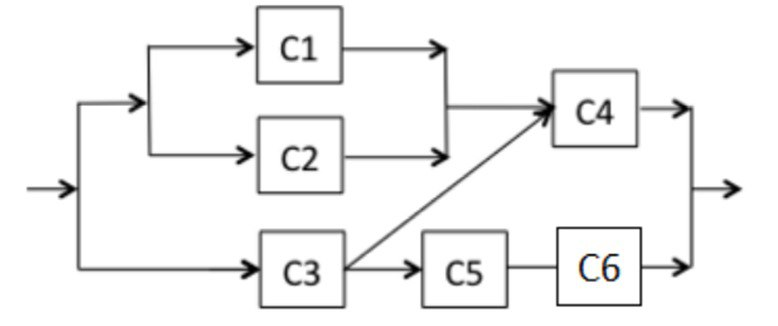
\includegraphics[width=0.8\textwidth]{img/ch5/ex1_traccia.png}
    \caption{RBD esercizio 1}
    \label{fig:ex1_traccia}
\end{figure}

Dallo schema in \cref{fig:ex1_traccia}, si osserva che il sistema non può essere ridotto ad un insieme di serie e parallelo a causa del collegmaento $C_3 \rightarrow C_4$. Pertanto, si è deciso procedere prima con la tecnica dell'\textit{upper bound} (\cref{eq:upper_bound_noserie_nopara}, dove con $R_{path}^i$ si indica la \textit{reliability} dell'i-esimo \textit{path} costituito dei componenti in serie del sistema.) e poi con quella del \textit{conditioning}.

\newpage
\subsection{Upper bound}
Applicando la formula in \cref{eq:upper_bound_noserie_nopara}:

\begin{equation}
    R_{sys} \leq 1 -\prod{(1 - R_{path}^i}) \
    \label{eq:upper_bound_noserie_nopara}
\end{equation}
, si calcola il limite superiore della reliability del sistema dato:

\begin{equation*}
    R_{sys} \leq 1 - [(1-R_1R_4) (1-R_2R_4) (1-R_2R_4) (1-R_3R_5R_6)]
\end{equation*}

Sostituendo i dati del problema si ottiene:

\begin{equation*}
    R_{sys} \leq 1 - [(1 - e^{-3 \lambda t}) (1 - e^{-2 \lambda t})^3]
\end{equation*}


\begin{figure}[H]
    \centering
    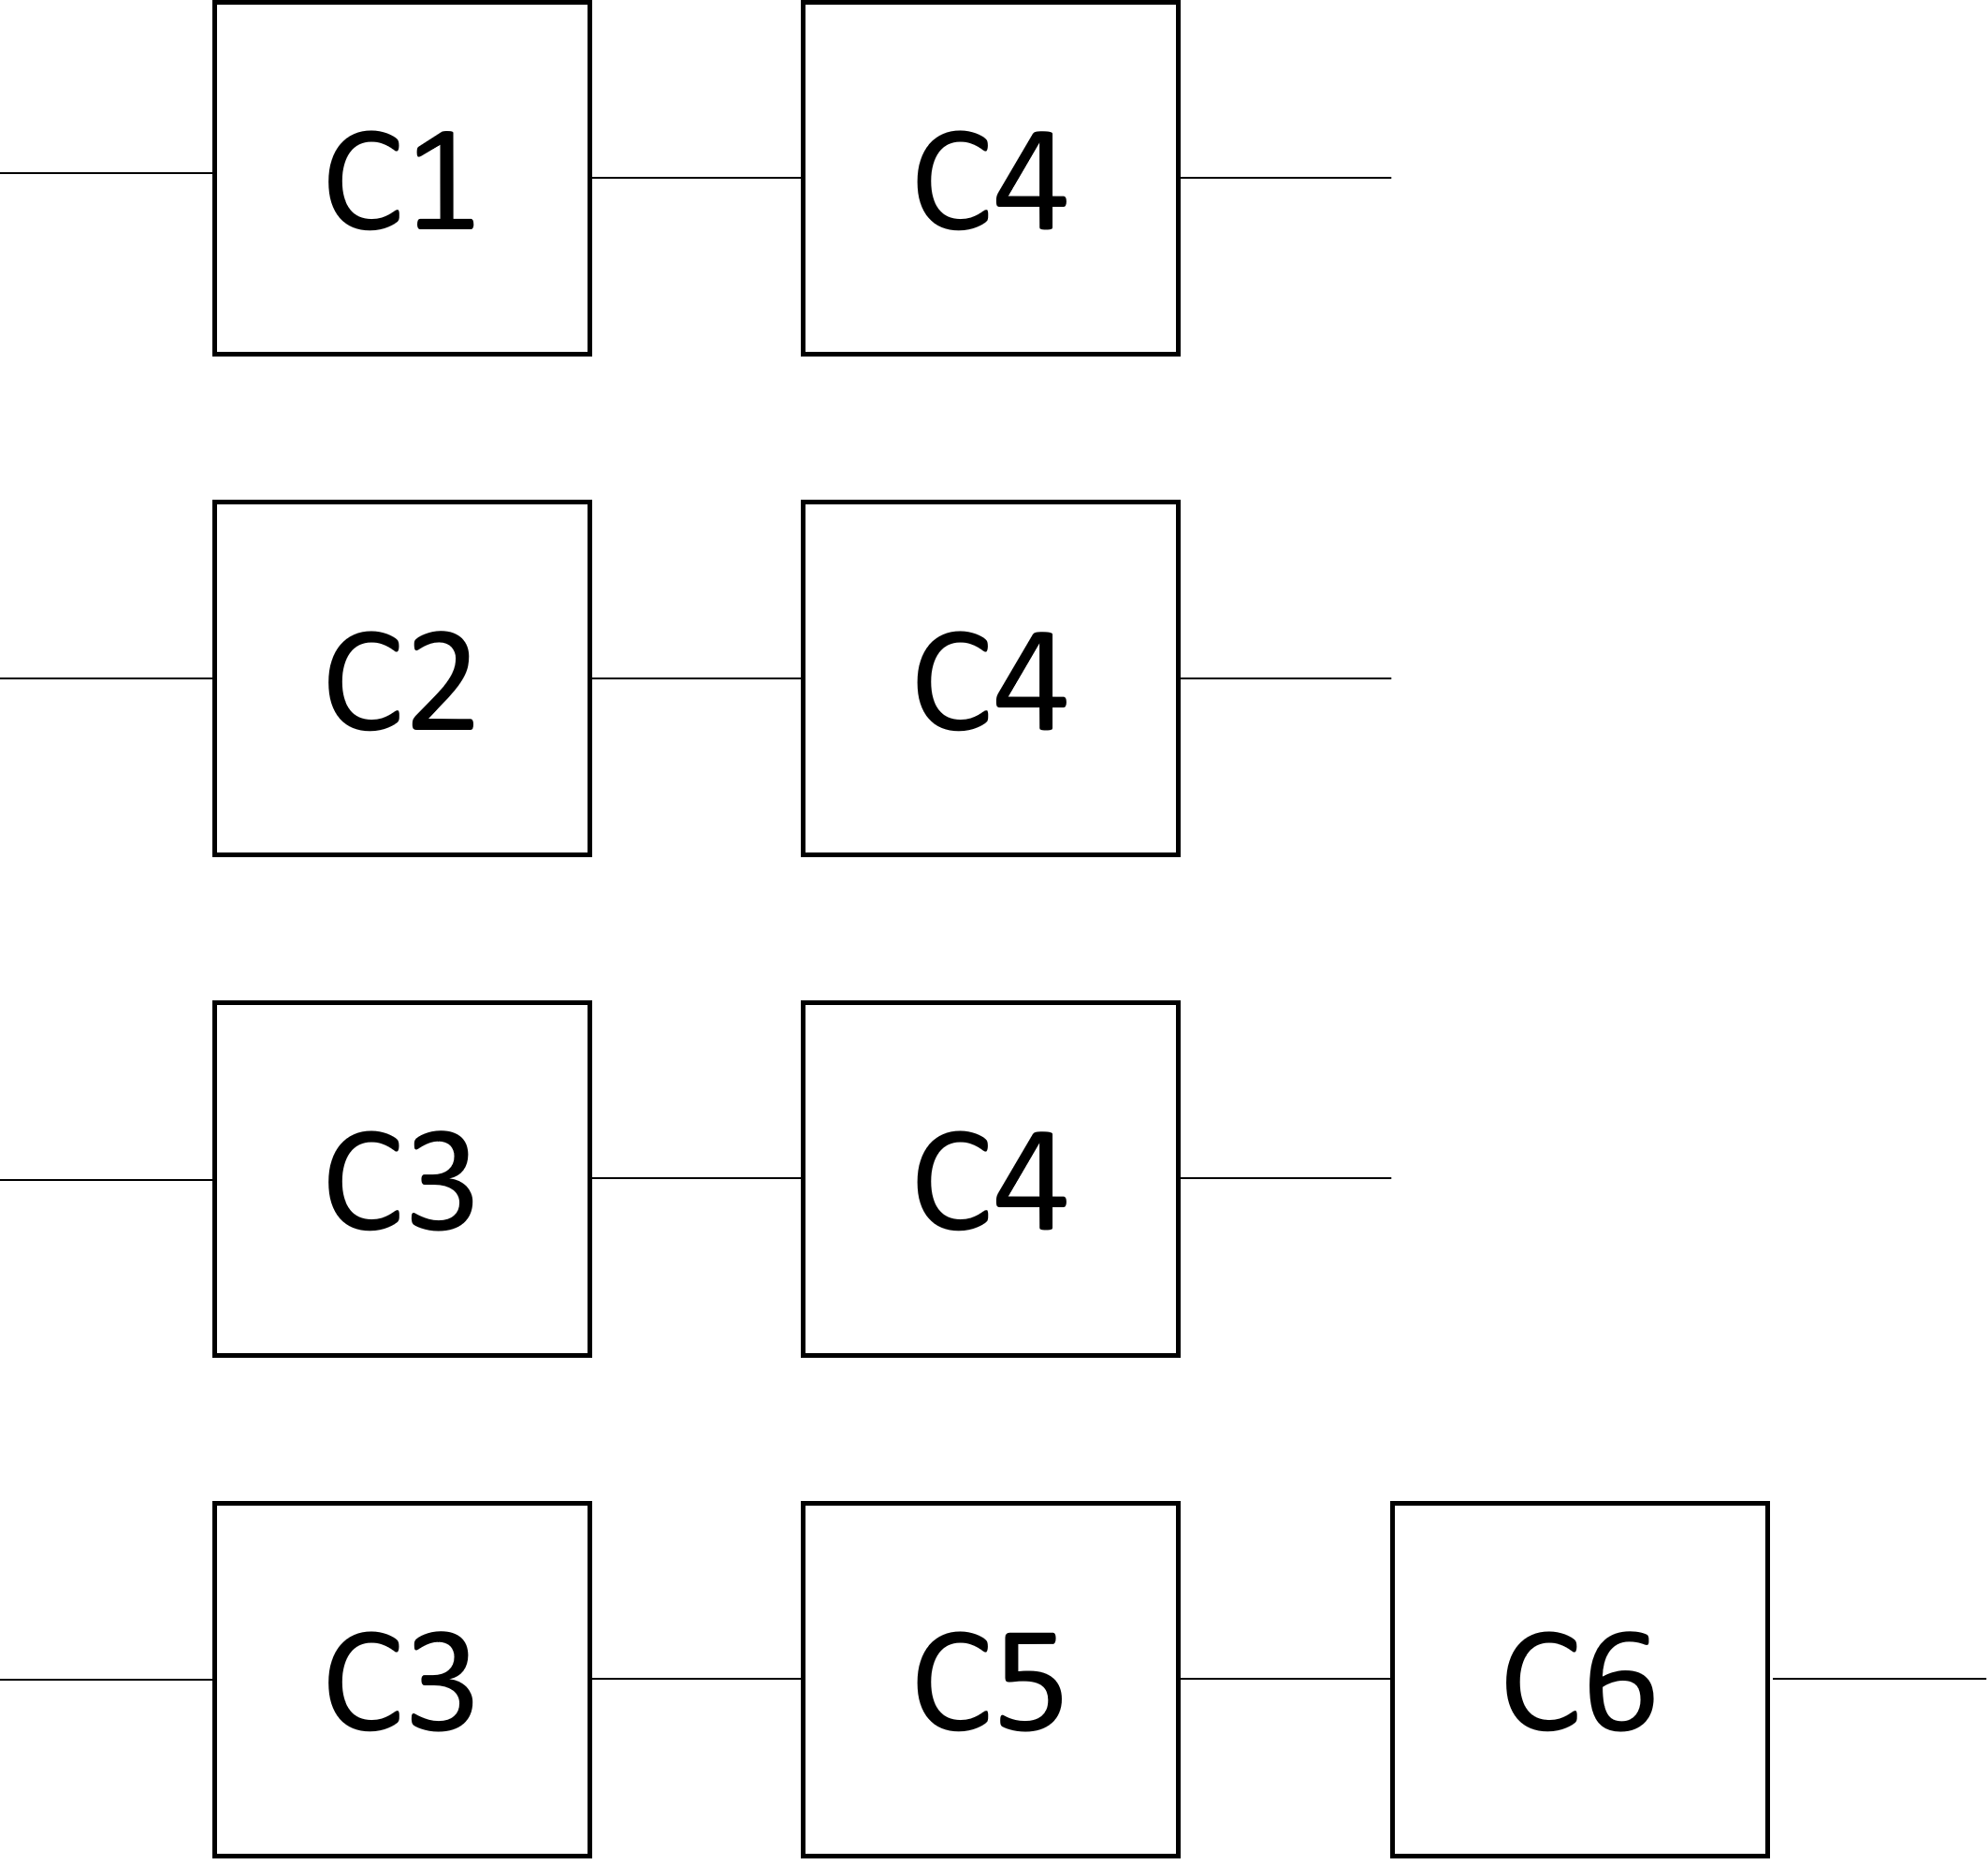
\includegraphics[width=0.5\textwidth]{img/ch5/upper_bound.png}
    \caption{Paths per l'upperbound}
    \label{fig:ex5_traccia}
\end{figure}

\newpage
\subsection{Conditioning}
Si è proceduto con l'analizzare il sistema quando il componente $C_3$ non funziona (assumendolo con un circuito aperto) e quando funziona (assumendolo con un cortocircuito) combinando i risultati mediante la probabilità totale. Quindi si ottiene:

\begin{equation*}
    R_{tot} = R_3 \cdot R_{C_3} + (1-R_3) \cdot R_{\overline{C}_3}
\end{equation*}

dove con $R_{C_3}$ si indica la \textit{reliability} del sistema laddove il componente $C_3$ funzioni; mentre con $R_{\overline{C}_3}$ si indica il sistema in cui $C_3$ non funzioni. Si risolvono i due diagrammi ottenuti \cref{fig:ex5_conditioning} in maniera indipendente.
\begin{figure}[H]
    \centering
    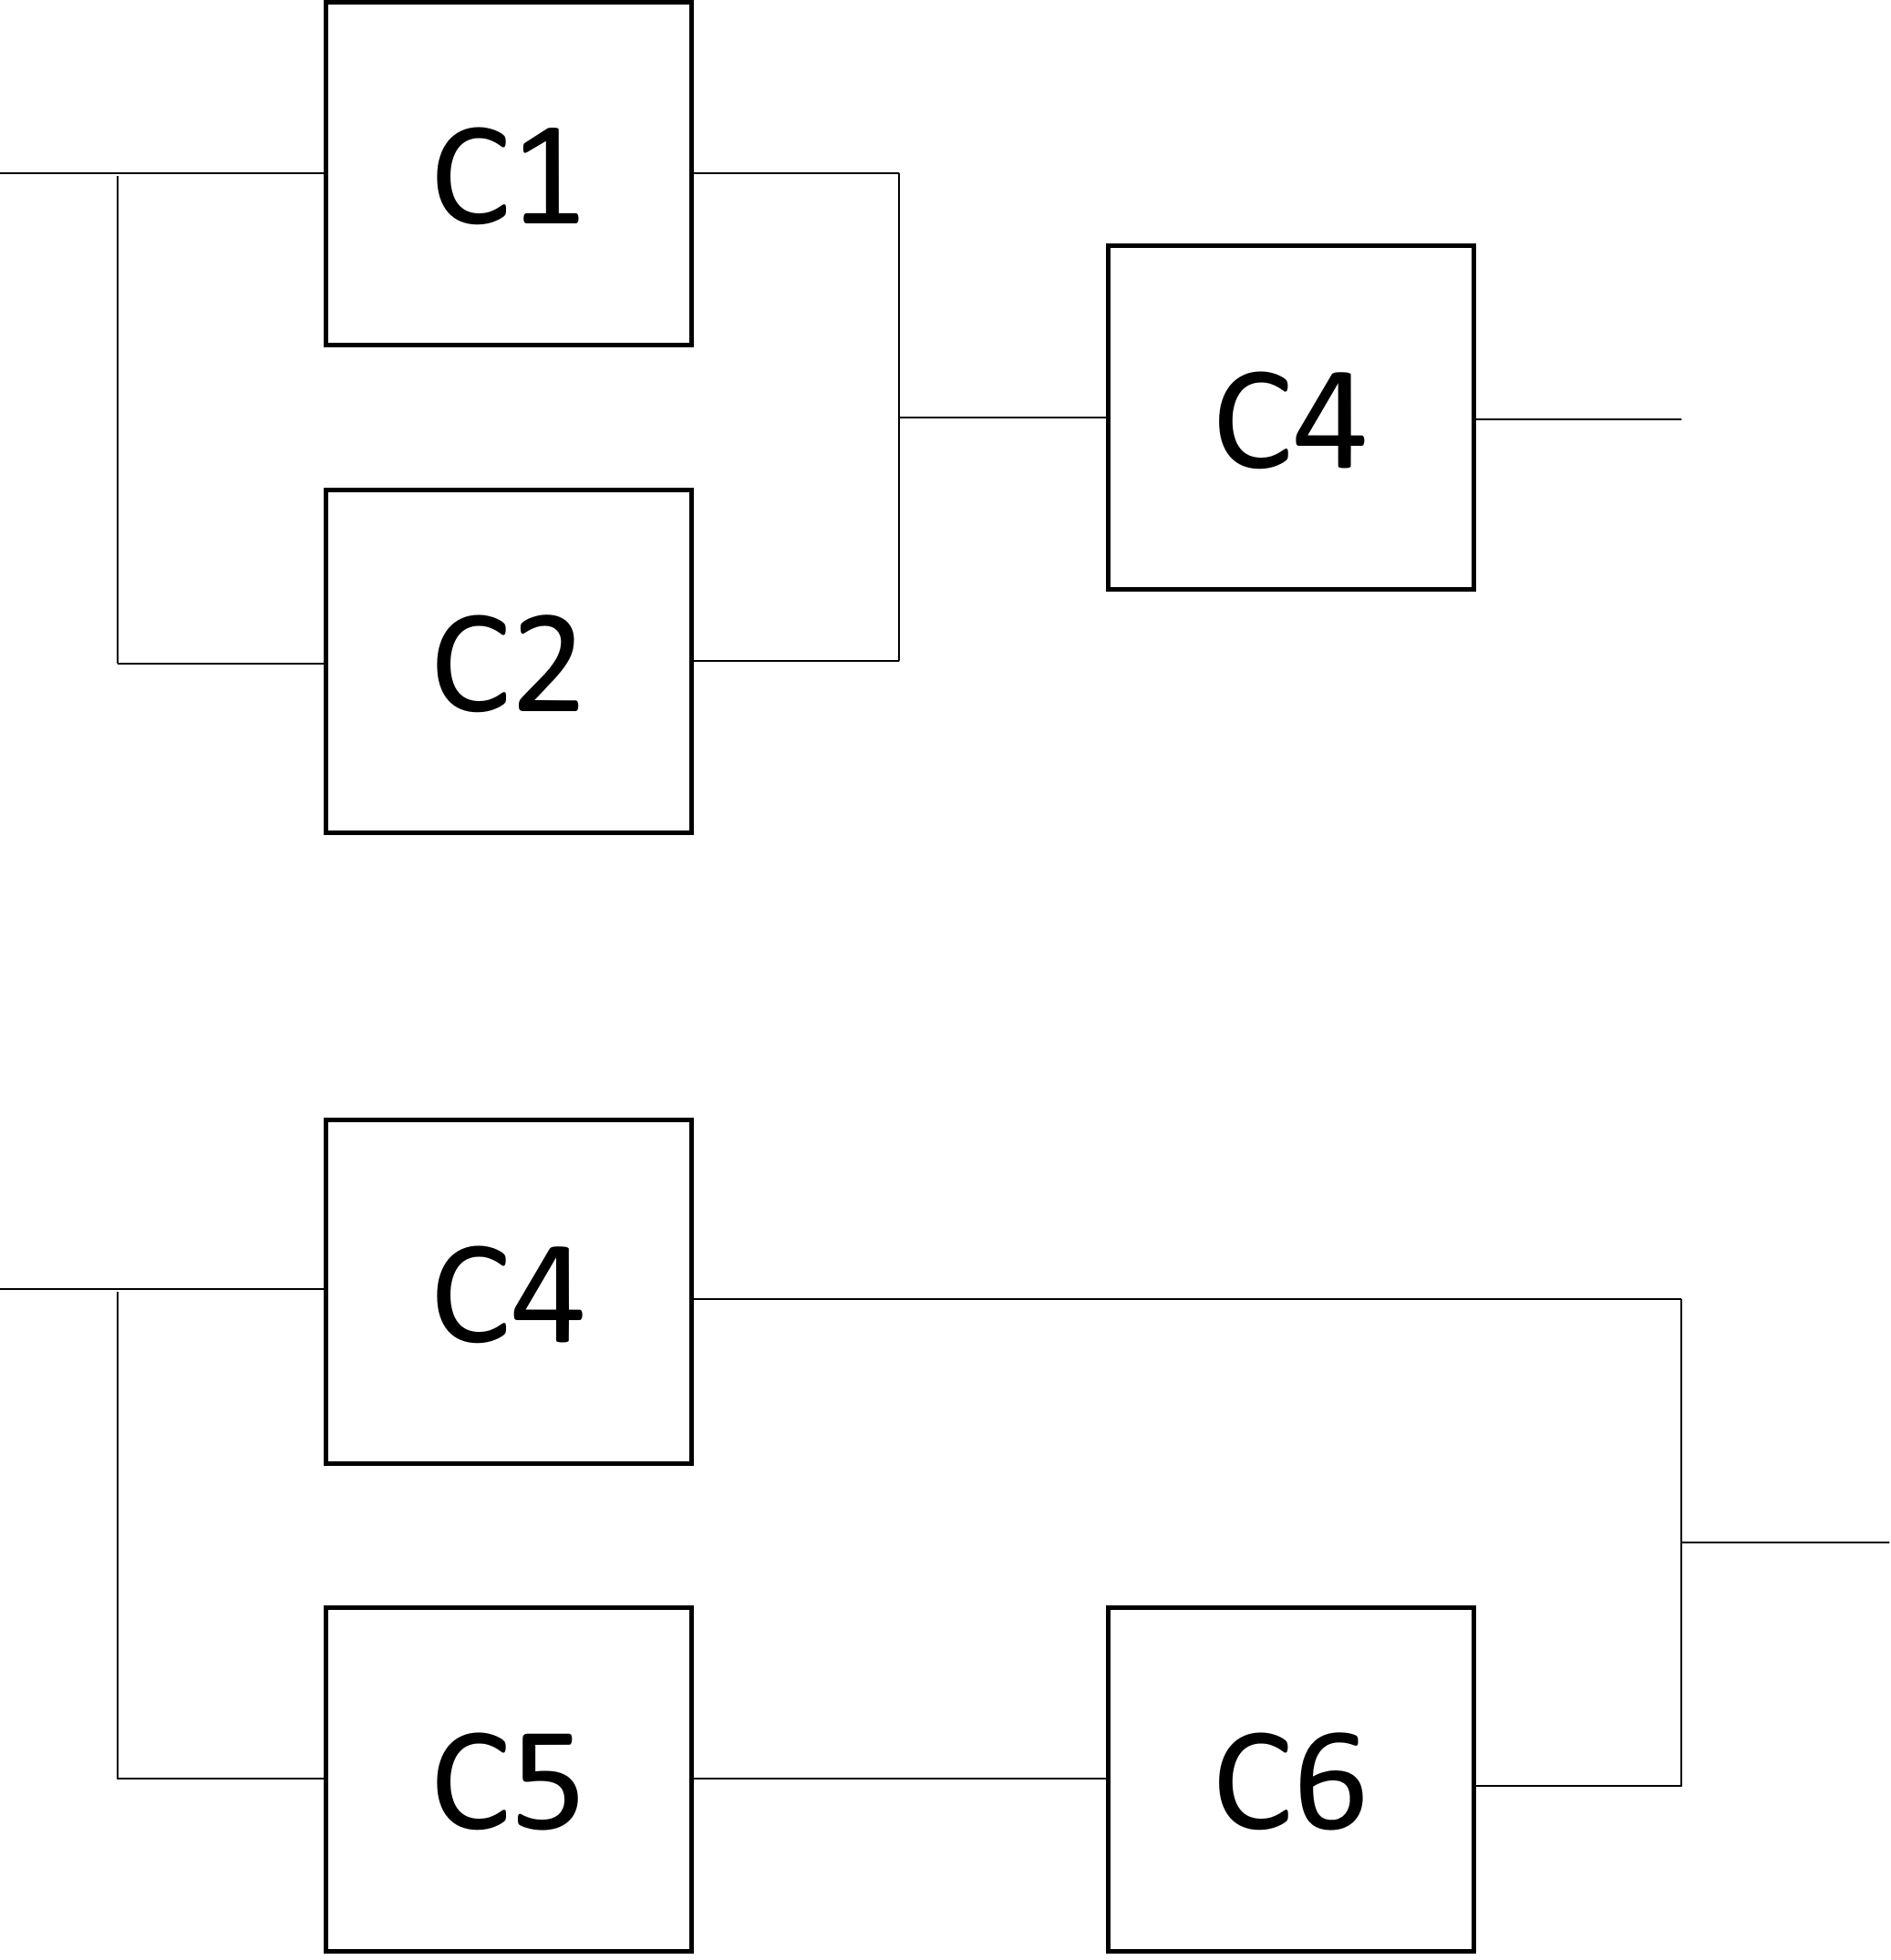
\includegraphics[width=0.5\textwidth]{img/ch5/conditioning.png}
    \caption{RBD con $C_3$ funzionante e non}
    \label{fig:ex5_conditioning}
\end{figure}

Nel caso in $C_3$ sia guasto, si ottiene:
\begin{equation*}
    R_{\overline{C}_3} = [1 - (1 - R_1) (1 - R_2)] R_4 = 2 e^{-2 \lambda t} - e^{-3 \lambda t}
\end{equation*}

Invece, quando $C_3$ funziona:

\begin{equation*}
    R_{C_3} = [1 - (1 - R_4) (1 - R_5R_6)] = -e^{-3 \lambda t} + e^{-2 \lambda t} + e^{-\lambda t}
\end{equation*}

Sostituendo i risultati ottenuti nell'espressione di $R_{tot}$:

\begin{align*}
    R_{tot} &= e^{-\lambda t} -e^{-3 \lambda t} + e^{-2 \lambda t} + e^{-\lambda t} + 2 e^{-2 \lambda t} - e^{-3 \lambda t} (1-e^{-\lambda t})\\
    &= -e^{-4 \lambda t} + e^{-3 \lambda t} + e^{-2 \lambda t} + e^{-4 \lambda t} - 3 e^{-3 \lambda t} + 2
    e^{-2 \lambda t} \\
    &= 3 e^{-2 \lambda t} - 2 e^{-3 \lambda t}
\end{align*}
\clearpage

\section{Exercise 2}
We want to compare two different schemes of increasing reliability of a system using redundancy. Suppose that the system needs s identical components in series for proper operation. Further suppose that we are given ($m x s$) components.  Given that the reliability of an individual component is R, derive the expressions for the reliabilities of two configurations. For $m = 2$ and $s = 4$, compare the two expressions as function of a mission time t.
Let MTTF of the component be $800$ hours.
Out of the two schemes shown in the figure below, which one will provide a higher reliability? Modify the scheme that has lower reliability in order to reach the same reliability of the other given the above MTTf ($800$ h).

\subsection{Calcolo e confronto della reliability dei due sistemi}
\begin{figure}[H]
    \centering
    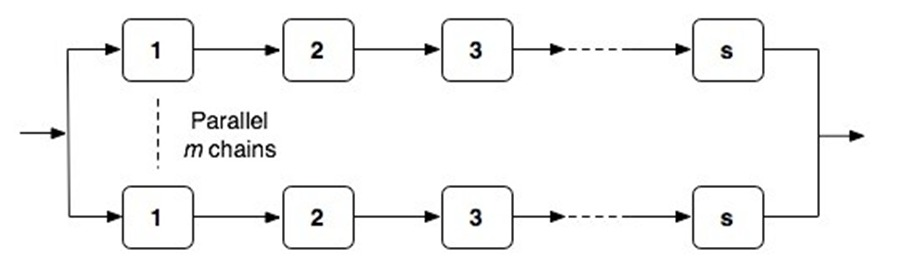
\includegraphics[width=0.8\textwidth]{img/ch5/exercise2.2.jpeg}
    \caption{Sistema 1}
    \label{fig:ex1_traccia}
\end{figure}

\begin{figure}[H]
    \centering
    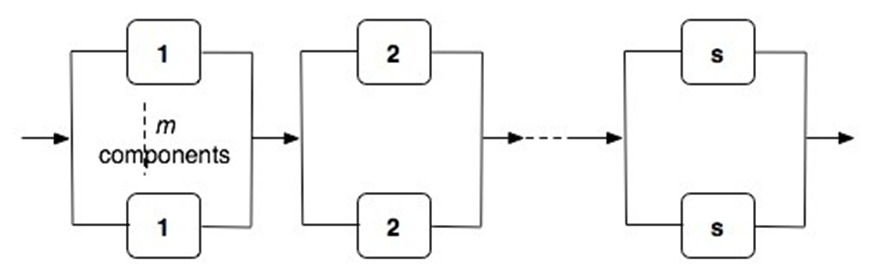
\includegraphics[width=0.8\textwidth]{img/ch5/exercise2.1.jpeg}
    \caption{Sistema 2}
    \label{fig:ex1_traccia}
\end{figure}

Per prima cosa sono state calcolate le reliability dei due sistemi, ottenute riducendoli in insiemi di serie e paralleli. In particolare, per il primo sistema ($m$ paralleli di $s$ serie) si è ottenuto il risultato in \cref{eq:m_sys1_res}; mentre per il secondo ($s$ serie di $m$ paralleli) si è ottenuto il risultato in \cref{eq:m_sys2_res}.

\begin{equation}
    R_{sys1} = 1 - (1 - R^s) ^ m
    \label{eq:m_sys1_res}
\end{equation}

\begin{equation}
    R_{sys2} = (1 - (1 - R)^m) ^ s
    \label{eq:m_sys2_res}
\end{equation}

Per $m=2$ e $s=4$, si ottiene:
\begin{equation*}
    R_{sys1} = 1 - (1 - R^4) ^ 2 = 1 - (1 - e{^{-4\lambda t}}) ^ 2
\end{equation*}
\begin{equation*}
     R_{sys2} = (1 - (1 - R)^m) ^ s = (1 - (1 - e{^{-\lambda t}})^2) ^ 4
\end{equation*}

Assegnato l'MTTF dei componenti uguale a 800 ore, quindi un  $\lambda=1/800$ sono stati tracciati i grafici relativi (mostrati in \cref{fig:ex5.2_comparazione}) alla reliability dei due sistemi al variare del tempo, da cui si evince che il sistema due sia più reliable del primo.

\begin{figure}[H]
    \centering
    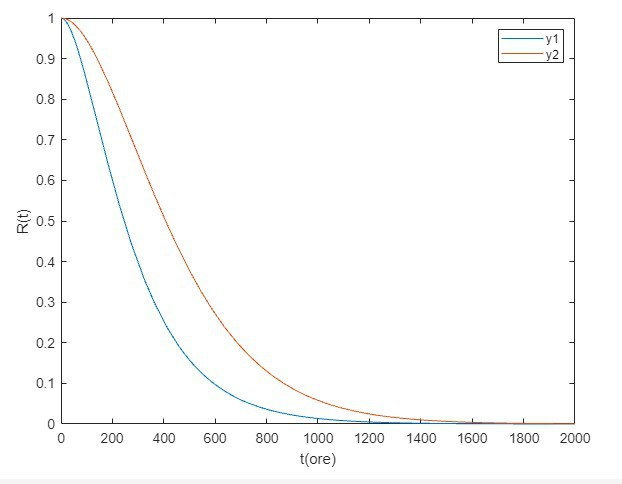
\includegraphics[width=0.8\textwidth]{img/ch5/comparison.png}
    \caption{Comparazione sistema 1 e sistema 2}
    \label{fig:ex5.2_comparazione}
\end{figure}


\subsection{Modifica del sistema 1}

Al fine di ottenere una reliability uguale a quella del sistema 2, si è fissato il tempo di missione per entrambi i sistemi a $800$ ore, facendo poi variare $m$ e ottenendo \cref{eq:ex5.2.3_soluzione}.

\begin{equation}
     0.1299 = 1 - (1-e^{-4\lambda t})^m; 
     \label{eq:ex5.2.3_soluzione}
\end{equation}

che ha come soluzione $ m \approx 7.53$, che approssimato per eccesso risulta essere $m=8$.

\begin{figure}[H]
    \centering
    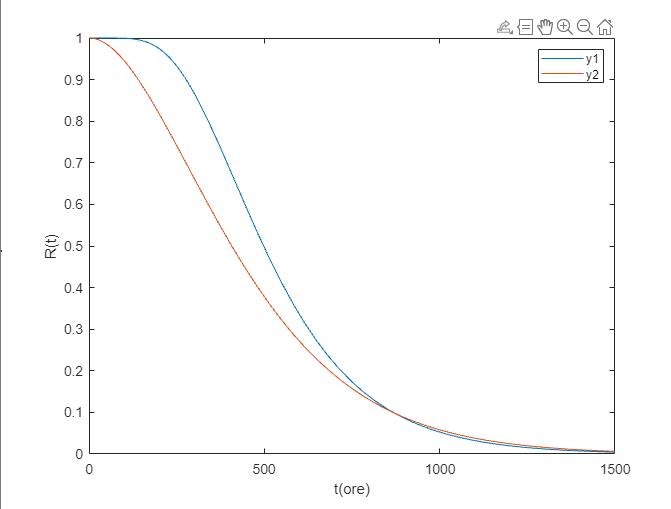
\includegraphics[width=0.8\textwidth]{img/ch5/s1_modified.png}
    \caption{Confronto \textit{reliability} tra $S_1$ modificato ($m=8$) $S_2$}
    \label{fig:ex5.2_comparazione}
\end{figure}

\clearpage
\section{Exercise 3}
The architecture of a network of computers in a banking system is shown below. The architecture is called a skip-ring network and is designed to allow processors to communicate even after node failures have occurred. For example, if node $1$ fails, node $8$ can bypass the failed node by routing data over the alternative link connecting nodes $8$ and $2$. Assuming the links are perfect and the nodes each have a reliability of $R_m$, derive and expression for the reliability of the network. If $R_m$ obeys the exponential failure law and the failure rate of each node is $0.005$ failures per hour, determine the reliability of the system at the end of a $48$-hour period.

\begin{figure}[H]
    \centering
    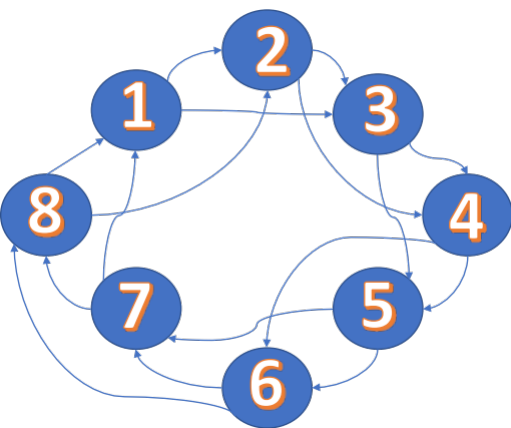
\includegraphics[width=0.5\textwidth]{img/ch5/3_traccia.png}
    \caption{Exercise 3}
    \label{fig:skip_ring}
\end{figure}

Partendo dalla topologia mostrata in \cref{fig:skip_ring} è stato ricavato il  fault tree in \cref{fig:fta_esercizio3}, che, come è possibile notare, presenta diversi eventi ripetuti.

\begin{figure}[H]
    \centering
    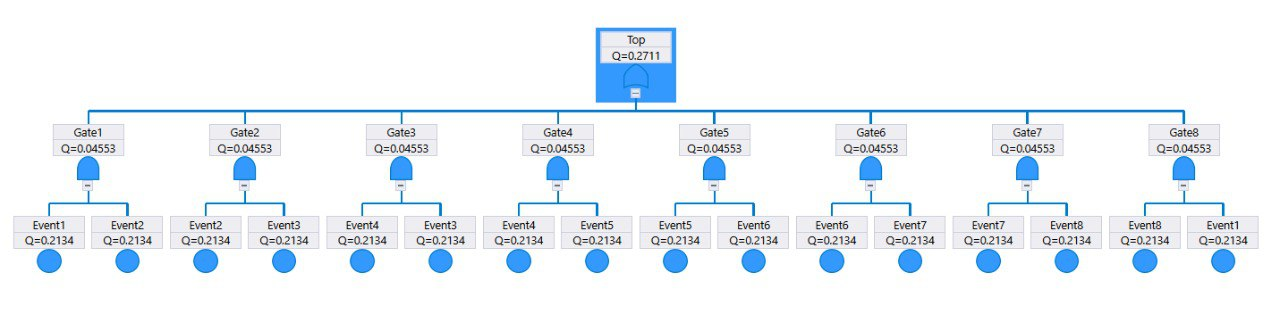
\includegraphics[width=\linewidth]{img/ch5/fta_esercizio3.png}
    \caption{Fault tree ricavato dalla \textit{skip ring network}}
    \label{fig:fta_esercizio3}
\end{figure}

A causa degli eventi ripetuti non è stato possibile convertire il fault tree in un RBD per calcolare la reliability.

È stato quindi utilizzato il metodo BDD, che converte i fault tree in Binary Decision Diagrams. Questi rappresentano l'equazione booleana che descrive il top event. Le probabilità possono quindi essere calcolate direttamente col BDD. 

Per farlo ci si è avvalsi del software \textit{TopEventFTA}, dove dopo aver costruito il Fault Tree, aver inserito le reliability dei componenti e fissando il tempo di missione a $48$ ore, la reliability del sistema risulta essere $0.728882$ .


\clearpage
\section{Exercise 4}
Compare the reliability of the following schemes, assuming an exponential failure occurrence with following values:
\begin{itemize}
    \item $MTTF_a=500$;
    \item $MTTF_b=9000$;
    \item $MTTF_c=1000$;
\end{itemize}

\begin{figure}[H]
    \centering
    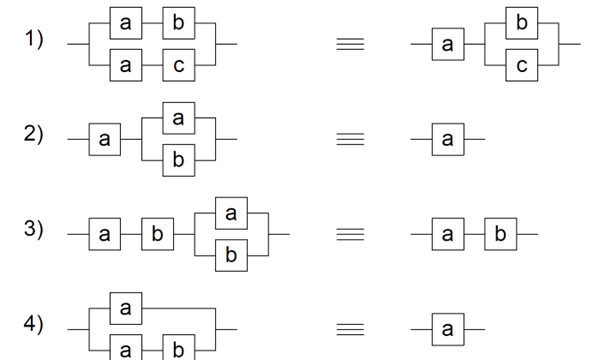
\includegraphics[width=0.8\textwidth]{img/ch5/exercise_4.png}
    \caption{Exercise 4}
    \label{}
\end{figure}

\paragraph{Punto 1}

Sono state calcolate le reliability per i due schemi, $y_1$ e  $y_2$, e ne è stato fatto il confronto in \cref{fig:4.1_cmp}.

\begin{itemize}
    \item $y_1  = 1-(1 - R_aR_b) \cdot (1 - R_aR_c)$
    \item $y_2  = R_a\cdot(1 - (1-R_b)) \cdot (1 - R_c)$
\end{itemize}

\begin{figure}[H]
    \centering
    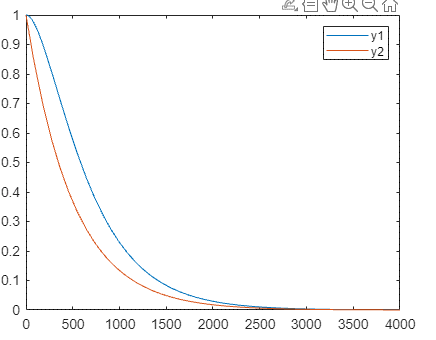
\includegraphics[width=0.8\textwidth]{img/ch5/4.1.png}
    \caption{Comparazione reliability punto 1}
    \label{fig:4.1_cmp}
\end{figure}

Si osserva che nello schema a destra il componente $a$ si comporta da \textit{single point of failure} per il sistema. In quello a sinistra, essendoci un parallelo e due copie di $a$ il sistema risulta più \textit{reliable}.

\paragraph{Punto 2}

Sono state calcolate le reliability per i due schemi, $y_1$ e  $y_2$, e ne è stato fatto il confronto in \cref{fig:4.2_cmp}.

\begin{itemize}
    \item $y_1  = R_a\cdot(1 - (1-R_b) \cdot (1 - R_a))$
    \item $y_2  = R_a$
\end{itemize}

\begin{figure}[H]
    \centering
    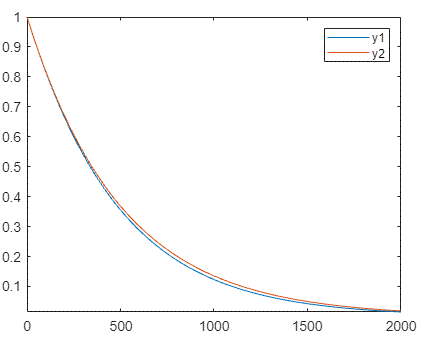
\includegraphics[width=0.8\textwidth]{img/ch5/4.2.png}
    \caption{Comparazione reliability punto 2}
    \label{fig:4.2_cmp}
\end{figure}
Si osserva che, prevedibilmente, il sistema 2 ha una reliability più alta. Il sistema a sinistra è infatti una serie di componenti di cui A fa parte, e avrà per forza una reliability generica del tipo $Ra\cdot R_i$ (dove $R_i$ corrisponde alla reliability del resto della serie) che essendo un prodotto di probabilità sarà sicuramente $\leq Ra$.


\paragraph{Punto 3}

Sono state calcolate le reliability per i due schemi, $y_1$ e  $y_2$, e ne è stato fatto il confronto in \cref{fig:4.3_cmp}.

\begin{itemize}
    \item $y_1  = R_aR_b\cdot(1 - (1-R_b) \cdot (1 - R_a))$
    \item $y_2  = R_aR_b$
\end{itemize}

\begin{figure}[H]
    \centering
    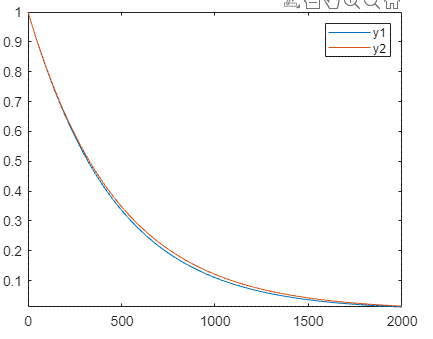
\includegraphics[width=0.8\textwidth]{img/ch5/4.3.png}
    \caption{Comparazione reliability punto 3}
    \label{fig:4.3_cmp}
\end{figure}
Si osserva che, prevedibilmente, il sistema 2 ha una reliability più alta. Il sistema a sinistra è infatti una serie di componenti di cui A-B fa parte, e avrà per forza una reliability generica del tipo $Rab\cdot R_i$ (dove Ri corrisponde alla reliability del resto della serie) che essendo un prodotto di probabilità sarà sicuramente $\leq Rab$.


\paragraph{Punto 4}

Sono state calcolate le reliability per i due schemi, $y_1$ e  $y_2$, e ne è stato fatto il confronto in \cref{fig:4.4_cmp}.

\begin{itemize}
    \item $y_1 = 1-((1 - R_a) \cdot (1 - R_bR_a))$
    \item $y_2 = R_a$
\end{itemize}

\begin{figure}[H]
    \centering
    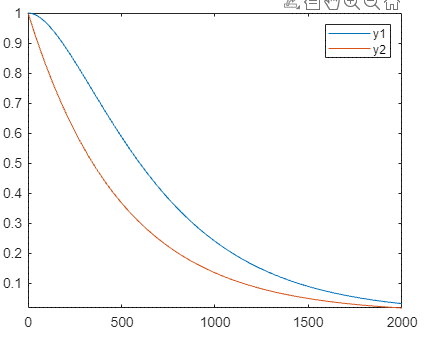
\includegraphics[width=0.8\textwidth]{img/ch5/4.4.png}
    \caption{Comparazione reliability punto 4}
    \label{fig:4.4_cmp}
\end{figure}

Il sistema a sinistra risulta più affidabile di quello di destra. Si può osservare come, al netto del componente B, il sistema a sinistra risulta un parallelo di componenti A e che la presenza di B peggiora solo la reliability. In questo caso però, dato che l'MTTF di B è di un ordine di grandezza superiore a quello di A il suo impatto è marginale.

\newpage
\section{Exercise 5}
The system shown in the figure below is a processing system for a helicopter. The system has dual-redundant processors and dual-redundant interface units. Two buses are used in the system, and each bus is also dual-redundant. The interesting part of the system is the navigation equipment. The aircraft can be completely navigated using the Inertial Navigation System (INS). If the INS fails, the aircraft can be navigated using the combination of the Doppler and the altitude heading and reference system (AHRS). The system contains three AHRS units, of which only one is needed. This is an example of functional redundancy where the data from the AHRS and the Doppler can be used to replace the INS, if the INS fails. Because of the other sensors and instrumentation, both buses are required for the system to function properly regardless of which navigation mode is being employed. 

\begin{figure}[H]
    \centering
    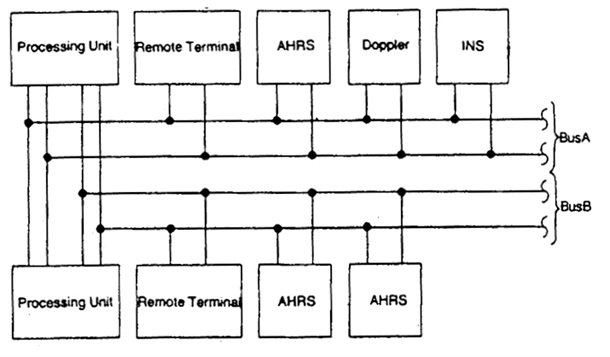
\includegraphics[width=0.8\textwidth]{img/ch5/exercise_5.png}
    \caption{Exercise 5}
\end{figure}

\begin{itemize}
    \item a) Draw the reliability block diagram of the system.
    \item b) Draw the Fault Tree of the system and analyze the minimal cutsets.
    \item c) Calculate the reliability for a one-hour flight using the MTTF figures given in the table below. Assume that the exponential failure low applies and that the fault coverage is perfect.
    \item d) Repeat (c), but this time, incorporate a coverage factor for the fault detection and reconfiguration of the processing units. Using the same failure data, determine the approximate fault coverage value that is required to obtain a reliability (at the end of one hour) of 0.99999.

\end{itemize}

\begin{figure}[H]
    \centering
    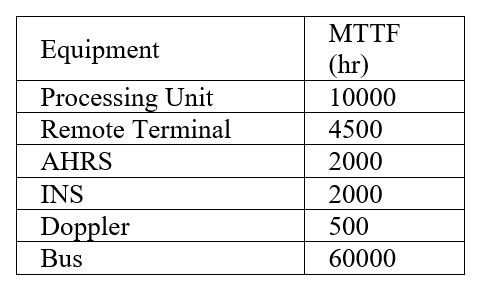
\includegraphics[width=0.5\textwidth]{img/ch5/tabella.png}
\end{figure}

\paragraph{Punto A}
Un \textit{RBD} è un diagramma che mostra il sistema dividendolo in più moduli, ognuno con una probabilità di funzionare $p$ o una reliability $R$, con lo scopo di calcolare la reliability generale.
Ogni modulo o componente è rappresentato solo una volta nel grafico, e i fallimenti sono indipendenti tra loro. Una volta fallito,si ritiene che il modulo darà sempre risultati sbagliati.

Il sistema inoltre verrà definito non funzionante quando non contiene un minimo set di moduli funzionanti, e una volta che entra nello stato di fallimento non potrà tornare a funzionare tramite altri fallimenti.

Per disegnare il \textit{reliability block diagram} sono state analizzate le relazioni tra i componenti, in modo da inserire in parallelo quelli ridondanti,e in serie quelli per cui un fallimento compromette il funzionamento del sistema.

In particolare, è possibile ridurre il sistema in più sottosistemi in serie, all'interno dei quali abbiamo diversi componenti in parallelo:
\begin{itemize}
    \item CPU: composto dal parallelo di CPU1 e CPU2
    \item BUS A: composto dal parallelo di BusA1 e BusA2
    \item BUS B: composto dal parallelo di BusB1 e BusB1
    \item Sistema di navigazione: composto dal parallelo tra INS e una serie di Doppler e tre ASHRS3 in parallelo
    \item Terminale remoto: composto dal parallelo di Remote Terminal 1 e Remote Terminal 2
\end{itemize}

\begin{figure}[H]
    \centering
    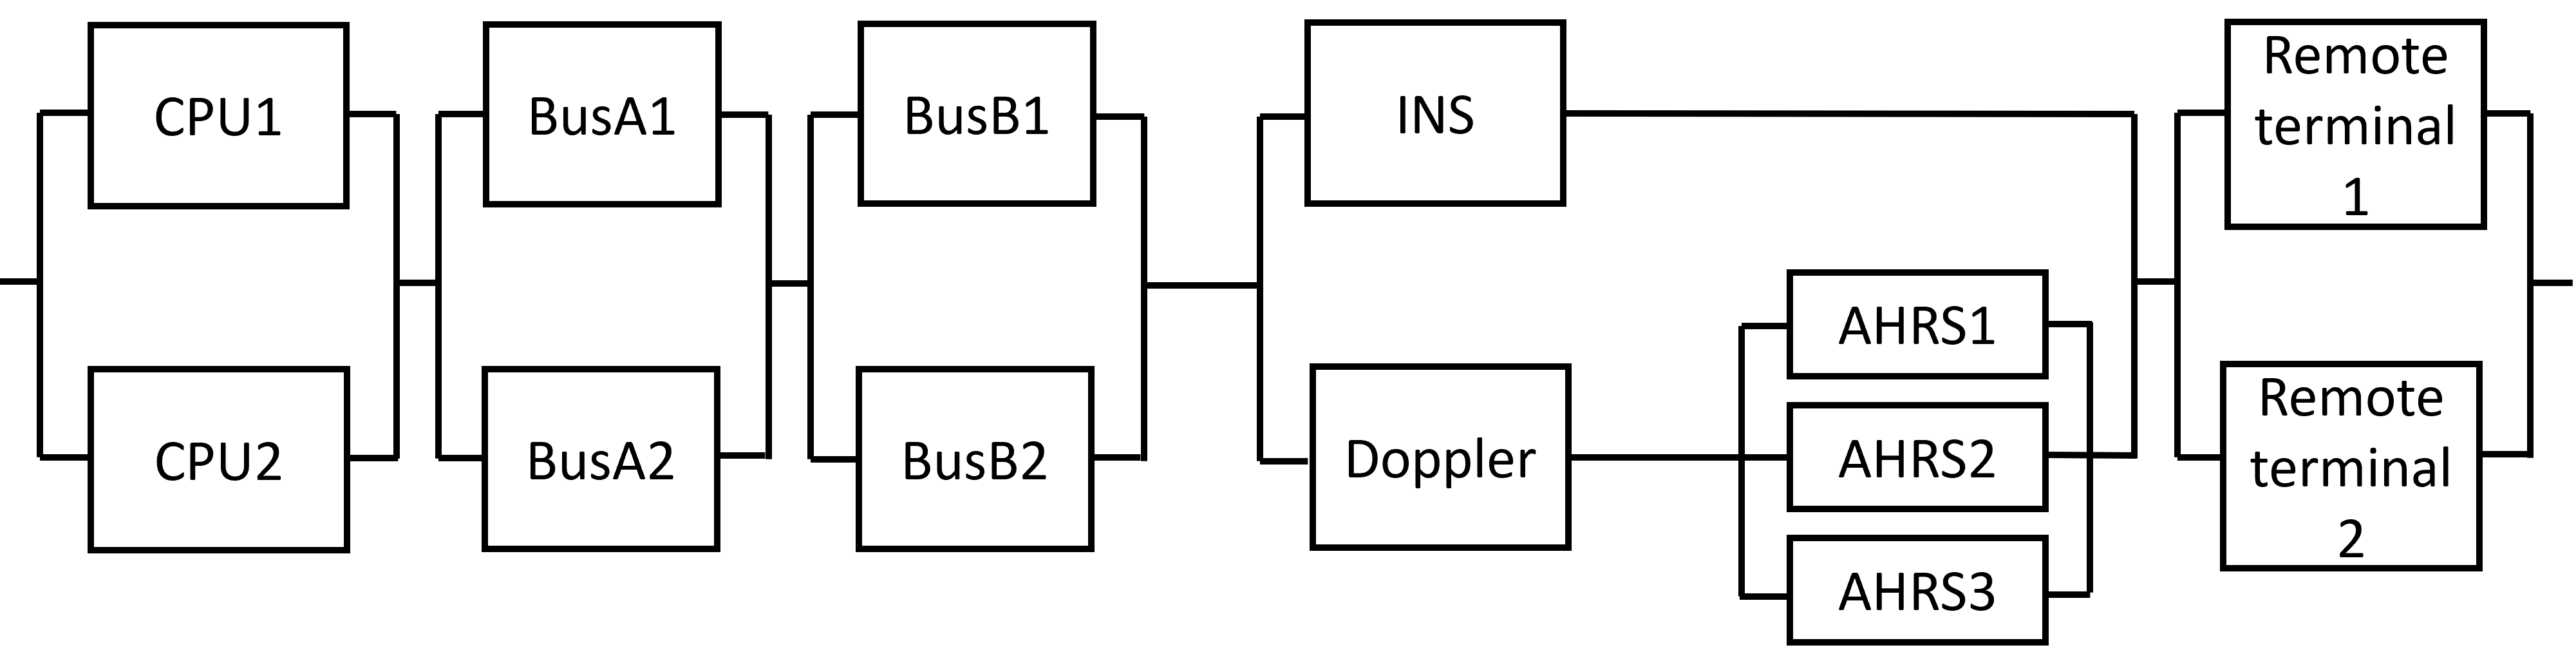
\includegraphics[width=0.8\textwidth]{img/ch5/helicopter_rbd.png}
    \caption{RBD del sistema}
    \label{fig:4.5_rbd}
\end{figure}

\paragraph{Punto B}
Un \textit{Fault Tree} è una rappresentazione grafica delle combinazioni di eventi che possono portare a un fallimento del sistema.
Le cause al più basso livello sono chiamati eventi base.
Ogni componente è rappresentato come un nodo, interconnesso con gli altri tramite porte logiche, e il fallimento di uno di questi porta l'input della porta a cui è collegato a diventare alto.

Per ottenere il \textit{fault tree} è possibile partire dal \textit{reliability block diagram} e trasformare le serie di componenti in una OR e i paralleli in \textit{AND}.

\begin{figure}[H]
    \centering
    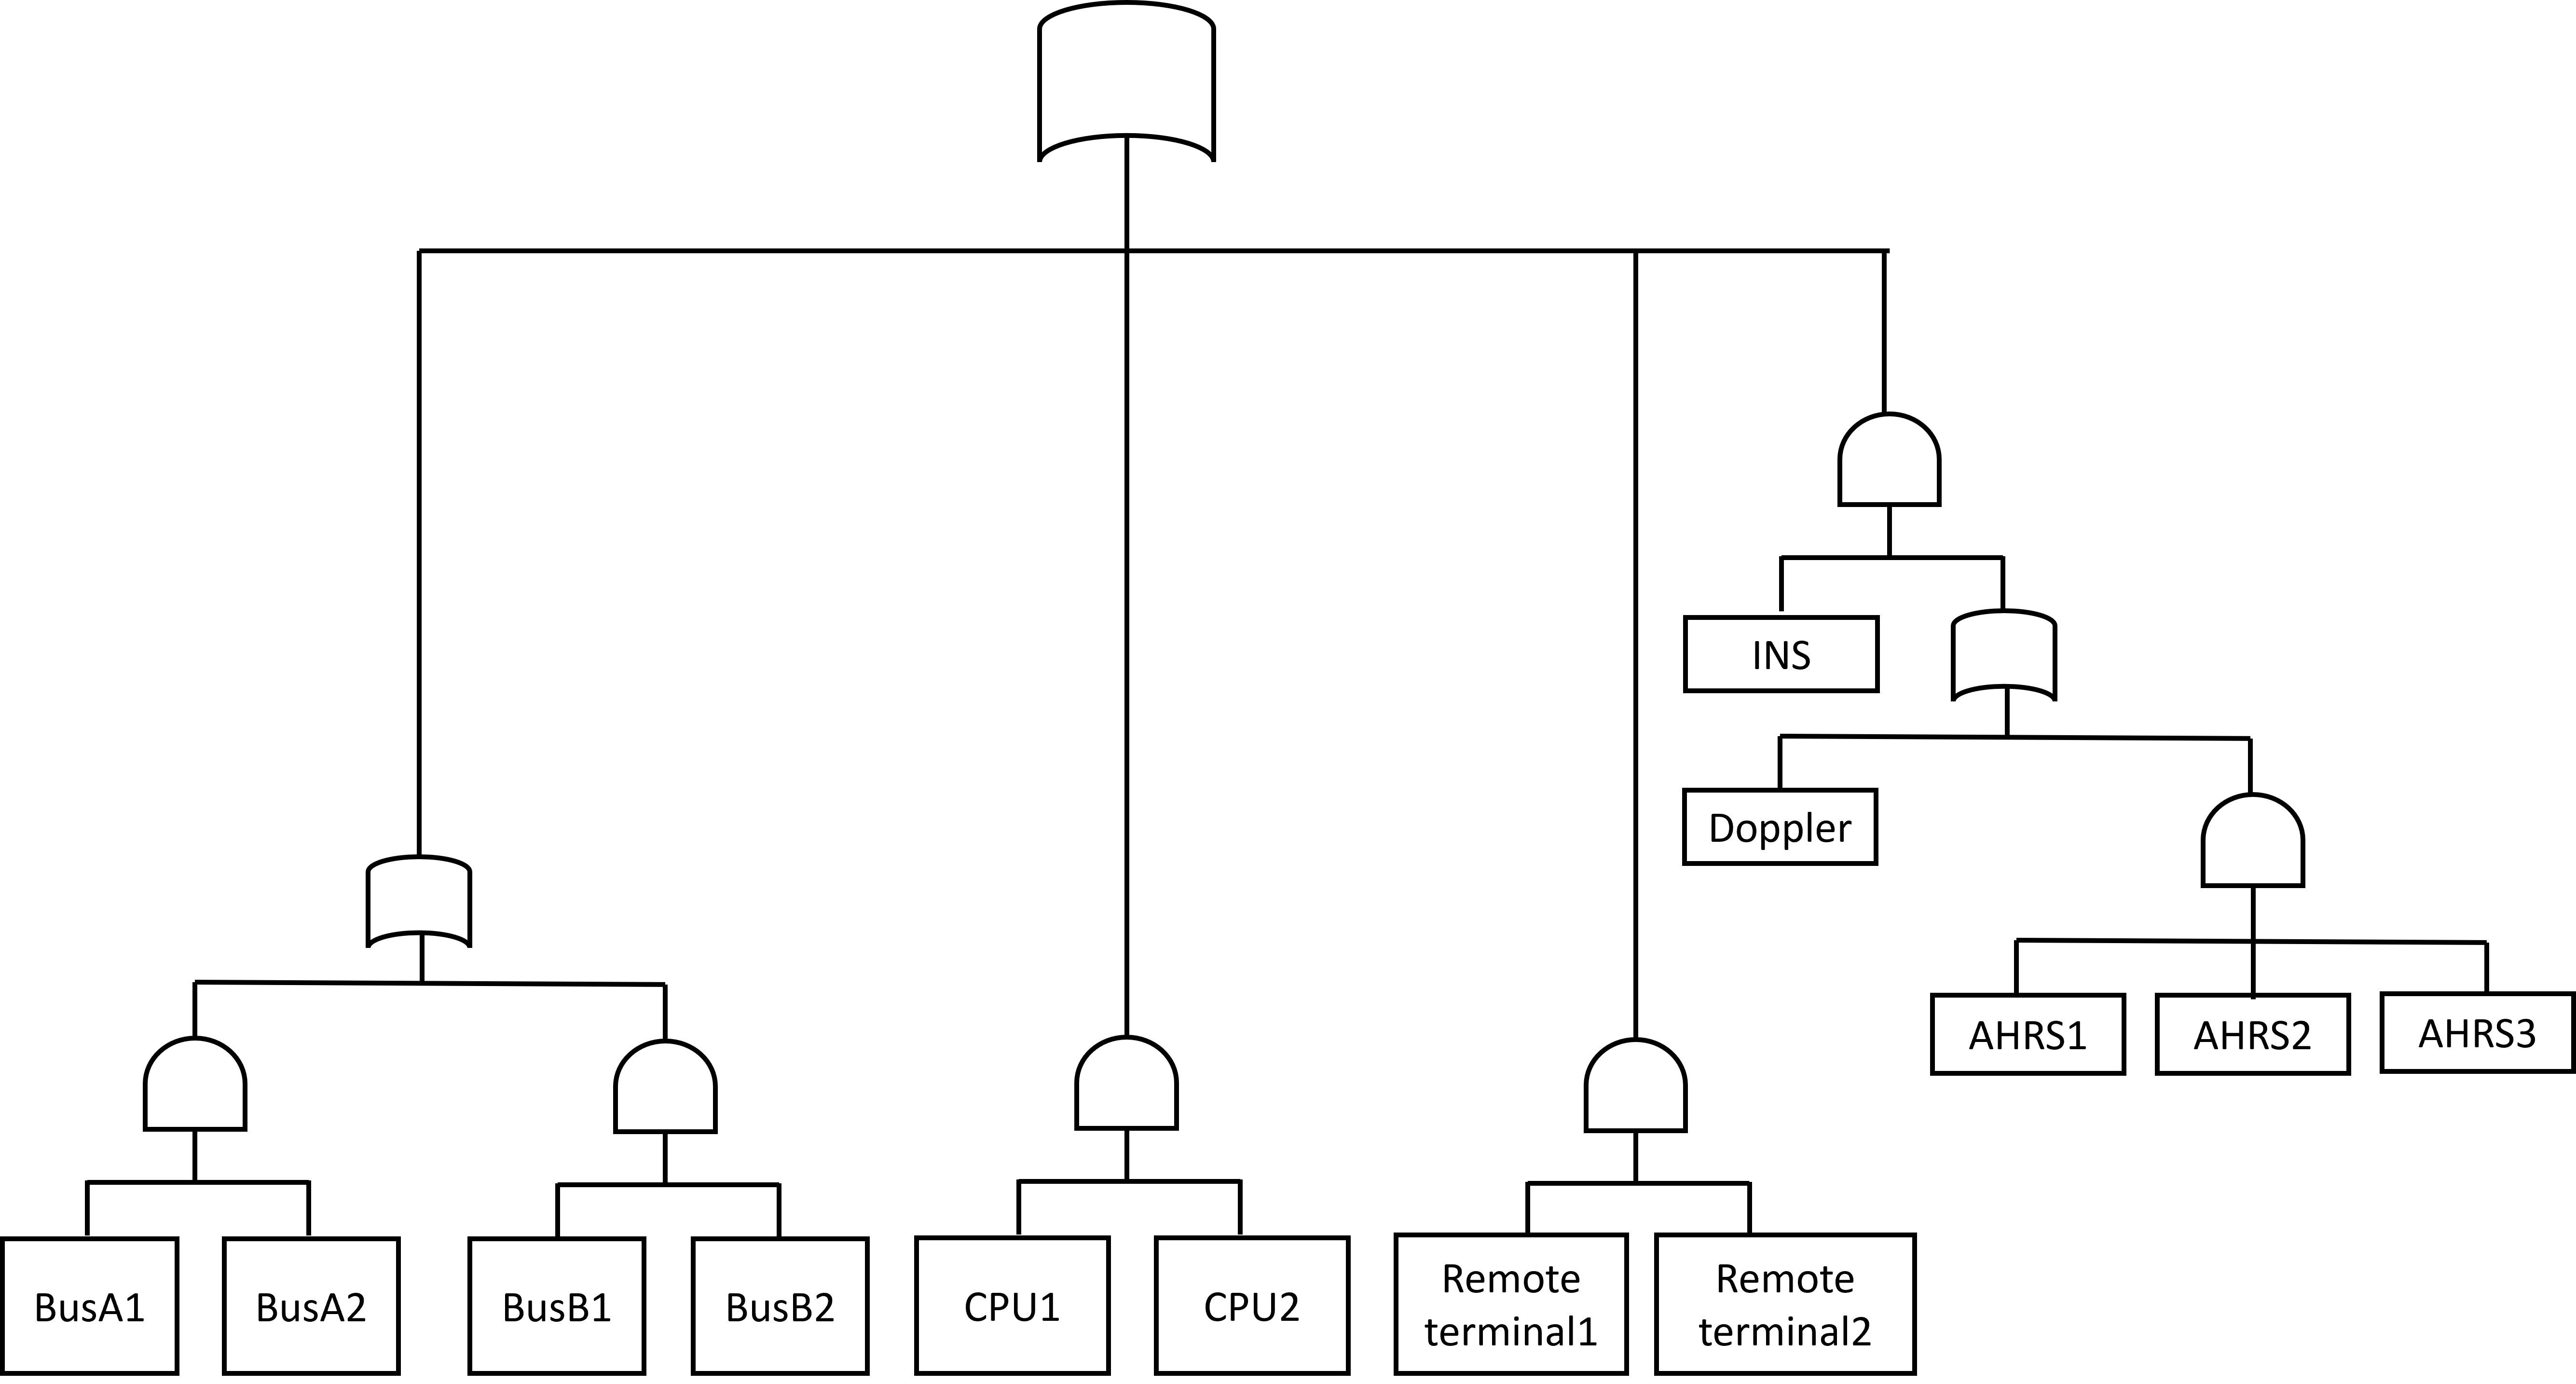
\includegraphics[width=0.8\textwidth]{img/ch5/fault_tree_helicopter.png}
    \caption{Fault tree del sistema}
    \label{fig:4.5}
\end{figure}

Il \textit{Minimal Cut Set} è definito come il più piccolo insieme di eventi base che, in congiunzione, possono causare il top level event, cioè il fallimento del sistema.
Di seguito sono mostrati i set trovati:
\begin{itemize}
    \item BUSA1 \land BUSA2
    \item BUSB1 \land BUSB2
    \item CPU1 \land CPU2
    \item Remote Terminal 1 \land Remote Terminal 2
    \item INS \land Doppler
    \item INS \land AHRS1 \land AHRS2 \land AHRS1 3
\end{itemize}

\paragraph{Punto C}
Partendo dall'RBD in \cref{fig:4.5_rbd} è possibile applicare le relazioni fondamentali di serie e parallelo. In particolare, si arriva alla relazione mostrata di seguito.

\begin{align*}
    R_{tot}&=(1-(1-R_{ter})^2) \cdot (1-(1-R_{cpu})^2)\\
    &\cdot(1-(1-R_{bus})^2)^2\cdot(1-(1-R_{ins})\\
    &\cdot(1-R_{dop}\cdot(1-(1-R_{ahrs})^3)))
\end{align*}

Sostituendo i dati del problema, si ottiene $R_{tot} = 0.99999894132275$.

\paragraph{Punto D}

La failure detection non è una tecnica perfetta, quindi nel caso di sistemi ridondati può essere possibile che un fault non venga rilevato. Questo possibile punto di fallimento del sistema viene modellato con l'introduzione di un componente $c$ in serie al sistema totale. Quindi, ad esempio, per un solo elemento ridondato, la reliability del parallelo è:
\begin{equation*}
    R = R_1 + c ( 1 - R_1)R_2
\end{equation*}
Nell'esercizio è richiesto di stimare il fattore $c$, immaginando di avere un fault detector non ideale solo per i componenti \textit{CPU1} e \textit{CPU2}, mantenendo una reliability pari a $0.99999$. Quindi, si è proceduto con riscrivere la relazione di \textit{reliability} utilizzando come incognita $c$.

\begin{align*}
    R_{tot}&=(1-(1-R_{ter})^2) \cdot (R_{cpu}+ c \cdot (1-R_{cpu}) \cdot R_{cpu}))\\
    \label{eq:rel_fault_coverage}
    &\cdot(1-(1-R_{bus})^2)^2\cdot(1-(1-R_{ins})\\
    &\cdot(1-R_{dop}\cdot(1-(1-R_{ahrs})^3)))
\end{align*}

Risolvendo l'equazione per $c$, si ottiene $c = 0.9106$.
